% Phase 3 handout -- RISC-V RV32I Single-Cycle CPU in Verilog
% EEL 4768 Computer Architecture, Fall 2026

\documentclass[11pt]{article}

\usepackage[letterpaper,margin=1in]{geometry}
\usepackage{amsmath,amssymb}
\usepackage{graphicx}
\usepackage{booktabs}
\usepackage{array}
\usepackage{multirow}
\usepackage{caption}
\usepackage{xcolor}
\usepackage{enumitem}
\usepackage{tikz}
\usetikzlibrary{arrows.meta,positioning,calc}
\usepackage{listings}
\usepackage[most]{tcolorbox}
\usepackage{fancyhdr}
\usepackage{parskip}
\usepackage[colorlinks=true,linkcolor=blue!50!black,urlcolor=blue!50!black]{hyperref}

\setlist[itemize]{topsep=2pt,itemsep=2pt,parsep=0pt}
\setlist[enumerate]{topsep=2pt,itemsep=2pt,parsep=0pt}

\lstset{
  basicstyle=\ttfamily\small,
  frame=single,
  breaklines=true,
  columns=fullflexible,
  keepspaces=true,
  showstringspaces=false,
  tabsize=4,
  backgroundcolor=\color{black!3}
}

\tcbuselibrary{skins,breakable}

\newtcolorbox{important}{
  colback=red!5!white, colframe=red!55!black, breakable,
  fonttitle=\bfseries, title=Note
}
\newtcolorbox{clarification}{
  colback=blue!5!white, colframe=blue!45!black, breakable,
  fonttitle=\bfseries, title=Clarification
}
\newtcolorbox{pitfall}{
  colback=orange!8!white, colframe=orange!65!black, breakable,
  fonttitle=\bfseries, title=Common Pitfall
}
\newtcolorbox{worked}{
  colback=green!5!white, colframe=green!35!black, breakable,
  fonttitle=\bfseries, title=Verilog Sketch
}
\newtcolorbox{example}{
  colback=green!5!white, colframe=green!35!black, breakable,
  fonttitle=\bfseries, title=Breakdown
}

\setlength{\headheight}{14pt}
\emergencystretch=1.5em

\pagestyle{fancy}
\fancyhf{}
\fancyhead[L]{EEL 4768 -- Computer Architecture}
\fancyhead[R]{Phase 3: Single-Cycle RV32I CPU}
\fancyfoot[C]{\thepage}
\renewcommand{\headrulewidth}{0.4pt}

\title{\vspace{-1.5cm}\textbf{Phase 3}\\[2pt]\Large Single-Cycle RV32I CPU}
\author{EEL 4768 Computer Architecture \\ Fall 2026}
\date{}

\begin{document}
\maketitle
\thispagestyle{fancy}
\vspace{-1cm}

\section*{Learning Objectives}
By the end of this phase you should be able to:
\begin{itemize}
  \item Assemble the blocks you built in Phase 2 into one working datapath.
  \item Design the full datapath of a single-cycle RV32I CPU.
  \item Validate a large, complex, multi-module design.
\end{itemize}


\begin{important}
You must write your own Verilog test benches to verify your designs. An example test trace will be provided, as well as a skeleton for \texttt{hart.v} in \texttt{phase\_3/skeletons/}.
\\
You also should reference the RV32I reference card from webcourses for the instruction formats, opcodes, and immediate values.
\end{important}

\section{Submission}
\begin{itemize}
  \item \textbf{One submission per group.} You will manually
        submit your work to Webcourses as a zip file. Students in multiple
        groups, or not in a group by the time of submission, will receive
        \textbf{no credit} for the submission.
  \item \textbf{Files to submit}:
\begin{lstlisting}
hart.v
alu.v
imm.v
rf.v
decoder.v
\end{lstlisting}
        One module per file, and name the module the same as the filename. The testbenches instantiate modules
        named \texttt{hart}, \texttt{alu}, \texttt{imm}, \texttt{rf} and
        \texttt{decoder} by name.
\end{itemize}

\section{Grading Rubric}
\label{sec:rubric}
\begin{center}
\begin{tabular}{@{}lr@{}}
\toprule
\textbf{Category} & \textbf{Points} \\
\midrule
Single-Cycle CPU & 5.0 \\
\midrule
\textbf{Total} & \textbf{5.0} \\
\bottomrule
\end{tabular}
\end{center}

\section{Verilog Coding Rules}
\label{sec:rules}
Your submission is internally checked against a synthesizable subset. This is to insure your code will be synthasizable for future phases. The rules listed below will result in a 0 for the specific file.

\begin{center}
\begin{tabular}{@{}p{5.4cm}p{8.8cm}@{}}
\toprule
\textbf{Rule} & \textbf{What it means for you} \\
\midrule
No \texttt{*}, \texttt{/}, \texttt{\%}, \texttt{**}
  & Arithmetic that does not synthesize cheaply. You do not need any of them
    in this phase. \\
No \texttt{===}, \texttt{!==}, \texttt{==?}, \texttt{!=?}
  & Not synthesizable. Use \texttt{==} and \texttt{!=}. \\
\textbf{Shifts only by a constant}
  & \texttt{x << 3} is fine; \texttt{x << i\_op2[4:0]} is \emph{rejected}. \\
No \texttt{if}/\texttt{else} in combinational logic
  & \texttt{if}/\texttt{else} is only legal inside a clocked
    \texttt{always @(posedge \dots)} block. For combinational logic use a
    continuous \texttt{assign} with the \texttt{?:} operator, or a
    \texttt{case} inside \texttt{always @(*)} (Valid for generate blocks on parameters and sequential logic only). \\
No procedural loops
  & \texttt{for}, \texttt{while}, \texttt{repeat} and \texttt{do}/\texttt{while}
    statements are rejected. To build something repetitive, use a
    \texttt{generate} loop, or just write the instances out. \\
No delays or waits
  & \texttt{\#5}, \texttt{wait}, \texttt{disable} and friends are simulation
    constructs. \\
No system tasks
  & \texttt{\$display}, \texttt{\$finish}, \texttt{\$stop}, \texttt{\$system},
    \texttt{\$readmemh}/\texttt{\$readmemb},
    \texttt{\$writememh}/\texttt{\$writememb} and all file I/O
    (\texttt{\$fopen}, \texttt{\$fwrite}, \dots) are not allowed in your final submission. Only
    constant functions such as \texttt{\$clog2} are allowed. \\
No \texttt{`include}
  & Not needed for importing other files. \\
\bottomrule
\end{tabular}
\end{center}

\newpage

\section{Single-Cycle CPU}
\label{sec:interface}
In phase 2, you designed and tested blocks that implement the ALU, register file, immediate generator and instruction decoder. In this phase, you will wire those blocks together into a single-cycle CPU that fetches, decodes, executes and writes back one instruction per clock cycle.

\begin{figure}[htbp]
\centering
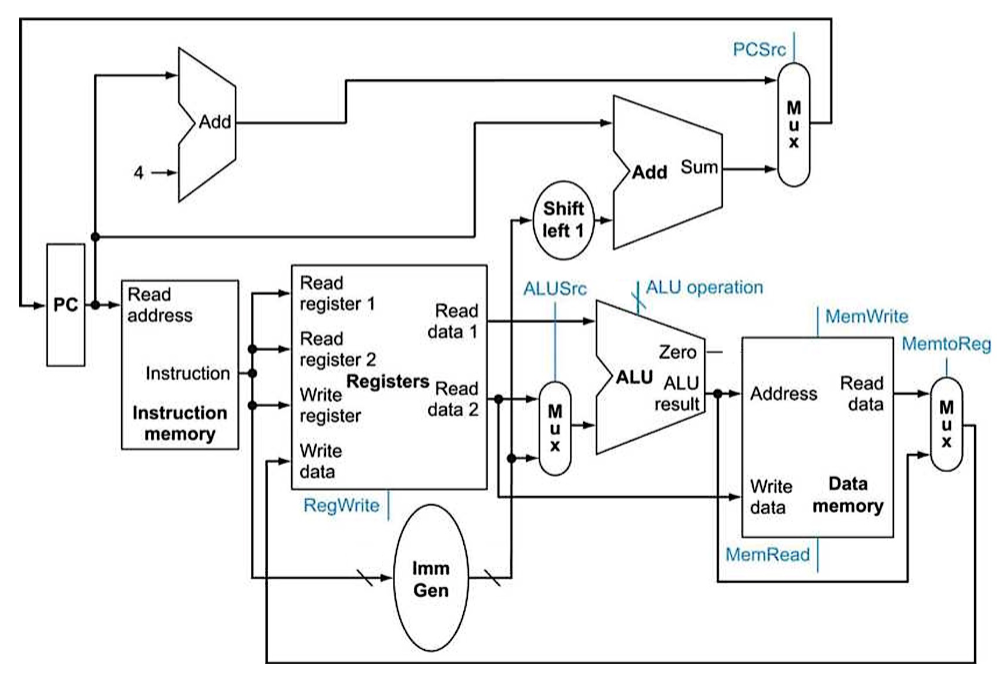
\includegraphics[width=0.95\textwidth]{image.png}
\label{fig:datapath}
\end{figure}

\begin{lstlisting}[language=Verilog]
module hart #(parameter RESET_ADDR = 32'h00000000) (
    input  wire        i_clk,
    input  wire        i_rst,
    /* ... */
);
\end{lstlisting}

\subsection{ALU, RF, Imm, and Decoder}
These modules will be reused from phase 2, and instantiated in \texttt{hart.v}. There are some small changes to the ALU and RF, which are described in Section~\ref{sec:instantiate}.

\subsection{PC}
In a processor, the program counter (PC) is a register that holds the address of the instruction to be fetched. You will need to implement a PC, which always points to the current instruction.

To go to the next instruction, the PC is either incremented by 4 (the size of an instruction in bytes), or set to a branch or jump target address. The PC is initialized to \texttt{RESET\_ADDR} on reset.

\subsection{Branch and jump}
Your processor will need to additionaly handle branching and jumping logic, which is used to overwrite the PC. When a branch or jump instruction is executed, the PC will be set to the target address. Otherwise, the PC will be incremented by 4.

\subsection{Instruction and data memory}
Besides the program counter and branch/jump logic, your CPU will need to handle the instruction and memory interfaces. Assume that the instruction and data memories are external to your design, and reading/writing requires no latency. Both are combinational, and require no clock edge to read or write. The instruction memory is read-only, while the data memory is read/write.

\begin{center}
\begin{tabular}{@{}llp{9.0cm}@{}}
\toprule
\textbf{Port} & \textbf{Dir/Width} & \textbf{Meaning} \\
\midrule
\texttt{o\_imem\_raddr} & out [31:0] & Instruction address. One instruction per cycle, always 4-byte aligned. \\
\texttt{i\_imem\_rdata} & in \ [31:0] & The instruction word at \texttt{o\_imem\_raddr}. \\
\texttt{o\_dmem\_addr}  & out [31:0] & Data address. \textbf{Always word-aligned.} \\
\texttt{o\_dmem\_ren}   & out        & Read enable. Never high in the same cycle as \texttt{o\_dmem\_wen}. \\
\texttt{o\_dmem\_wen}   & out        & Write enable. \\
\texttt{o\_dmem\_wdata} & out [31:0] & Store data. Only the lanes selected by \texttt{o\_dmem\_mask} are used. \\
\texttt{o\_dmem\_mask}  & out [3:0]  & Which of the four byte lanes of the word at \texttt{o\_dmem\_addr} are read or written. \\
\texttt{i\_dmem\_rdata} & in \ [31:0] & The full word at \texttt{o\_dmem\_addr}, regardless of mask. Extracting and sign- or zero-extending the right bytes is \texttt{hart.v}'s job. \\
\bottomrule
\end{tabular}
\end{center}

\begin{clarification}
\textbf{Sub-word accesses use the mask, not the address.} To pass a 32-bit word, all four lanes of \texttt{o\_dmem\_mask} must be high. See the comments on the \texttt{hart.v} skeleton for more details.
\end{clarification}

\subsection{Retire interface}
\label{sec:retire}
These outputs are not part of RV32I. They exist for the testbench to validate your design and its functionality. Set each signal appropriately every cycle. Because your design
is single-cycle, every fetched instruction retires in the cycle it is fetched:
\texttt{o\_retire\_valid} is high every cycle after \texttt{i\_rst} deasserts,
with no bubbles, through the cycle \texttt{o\_retire\_halt} fires.

\begin{center}
\begin{tabular}{@{}llp{9.0cm}@{}}
\toprule
\textbf{Port} & \textbf{Width} & \textbf{Meaning} \\
\midrule
\texttt{o\_retire\_valid}      & 1     & An instruction retired this cycle. \\
\texttt{o\_retire\_inst}       & [31:0]& The raw fetched instruction word. \\
\texttt{o\_retire\_trap}       & 1     & Illegal encoding, or a misaligned access. \\
\texttt{o\_retire\_halt}       & 1     & The instruction is \texttt{ebreak}. \\
\texttt{o\_retire\_rs1\_raddr} & [4:0] & Source register 1, \textbf{\texttt{5'd0} if not read}. \\
\texttt{o\_retire\_rs1\_rdata} & [31:0]& Value read from \texttt{rs1}. \\
\texttt{o\_retire\_rs2\_raddr} & [4:0] & Source register 2, \textbf{\texttt{5'd0} if not read}. \\
\texttt{o\_retire\_rs2\_rdata} & [31:0]& Value read from \texttt{rs2}. \\
\texttt{o\_retire\_rd\_waddr}  & [4:0] & Destination register, \textbf{\texttt{5'd0} if no register is written}. \\
\texttt{o\_retire\_rd\_wdata}  & [31:0]& Value written to \texttt{rd}. \\
\texttt{o\_retire\_pc}         & [31:0]& PC this instruction was fetched from. \\
\texttt{o\_retire\_next\_pc}   & [31:0]& \texttt{PC + 4}, or the branch or jump target when taken. \\
\bottomrule
\end{tabular}
\end{center}

\begin{important}
\textbf{Every field above is checked on every retiring instruction},
Make sure to handle these signals every cycle. Failure to do so will make your design not integrate with the testbench, and will result in a 0 for the entire phase.
\end{important}

\subsection{Instantiating your Phase 2 modules}
\label{sec:instantiate}
\begin{itemize}
  \item \textbf{\texttt{rf.v} is instantiated with \texttt{BYPASS\_EN = 0}.}
        In a single-cycle design an instruction's writeback commits on the
        same clock edge the next instruction's read samples, so there is no
        same-cycle read/write collision to bypass. Bypass will later be used in the pipelined datapath.
  \item \textbf{\texttt{decoder.v} already contains \texttt{imm.v}.} You
        instantiated it there in Phase 2; do not instantiate a second copy.
  \item \textbf{\texttt{alu.v} performs the branch comparison.} There is no
        separate comparator: \texttt{beq}, \texttt{bne}, \texttt{blt},
        \texttt{bge}, \texttt{bltu} and \texttt{bgeu} all read the ALU's
        \texttt{o\_eq} and \texttt{o\_slt} while \texttt{o\_result} is unused.
\end{itemize}

\begin{important}
\textbf{Phase 3 adds a small change to the ALU and RF.} 
\begin{itemize}
  \item You should additionally drive your ALU's \texttt{o\_sltu} when \texttt{i\_op} is \texttt{3'b011} (the \texttt{SLTU} instruction). This is the only change to your Phase 2 ALU.
  \item RF no longer contains \texttt{o\_rd\_wen}. Instead, gate instructions by setting the \texttt{i\_rd\_waddr} to \texttt{5'd0}.
\end{itemize}
For assistance making these changes, please come to office hours.
\end{important}

\newpage

\section{Testing Your Work}
\label{sec:testing}
\textbf{There is no autograder in this repository.} Verifying that
\texttt{hart.v} runs real programs correctly is part of the assignment. A
trace is provided in \texttt{phase\_3/traces/} that you can use to validate
your design. It is one continuously executing RV32I program of about
22{,}600 instructions, and it comes as two files rather than Phase 2's one:

\begin{itemize}
  \item \texttt{vectors/hart\_program.hex} --- the program itself, as a flat
        instruction memory image in \texttt{\$readmemh} format, one
        instruction per line, with the address being the line number times
        four. Your design fetches from it at whatever address it computes.
  \item \texttt{vectors/hart.trace} --- one line per instruction actually
        retired, in the order it happens, with one column per retire signal.
        Nothing in it is driven into your design; it is only compared
        against. A column written as \texttt{x} is a don't-care.
\end{itemize}

\subsection{Running it}
Put your Verilog in \texttt{phase\_3/traces/submission/} and run
\texttt{./run\_traces.sh}, or point it at wherever your files already live:

\begin{lstlisting}[language={}]
$ ./run_traces.sh ~/eel4768/phase_3
...
[FAIL] vector 9645 (LOAD_STORE.SB_LB): pc=000096b0 inst=009f8123
         mem_wdata lane 3: got ff, expected 2a
...
---------- summary ----------
vectors: 22661   passed: 22600   failed: 61
  LOAD_STORE.SB_LB  300/360 <-- FAIL

TEST FAILED: 61 of 22661 vectors wrong.
\end{lstlisting}

Each failure names the signal that disagreed and the instruction it
disagreed on. The full output and the compile log are left in
\texttt{traces/build/hart/}. You need \texttt{iverilog} and \texttt{vvp};
nothing else.

\end{document}
